\chapter{干细胞、再生与衰老}\label{ch:b3:stem-cells}

切掉一只墨西哥钝口螈的一条腿，两个月后它便长出一条新腿，
骨骼、肌肉、神经与皮肤各归其位，且可以
反复\omterm{def:b3:stem-cells:regeneration}{再生}，切多少次就\omterm{def:b3:stem-cells:regeneration}{再生}多少次。把一条涡虫切成二十段，
每段都在两周内长成一条完整的涡虫，原为尾部的那一段
长出带眼睛和脑的头。切掉人的手指，
若在最后一个关节以上切断，则只会愈合为疤痕。然而人体
并非没有更新：每秒钟生成 200 万个血
细胞，肠道内壁每五天更换一次，皮肤
每月更换一次，而这一切都源于少量细胞群体，
这些细胞终生不断分裂而不耗尽自身。本
章讨论这些细胞——什么使一个细胞成为\omterm{def:b3:stem-cells:stem}{干细胞}，其\omterm{def:b3:stem-cells:stem}{生态位}如何维持它，
以及血液或肠道的整个层级如何由它构建而成——
讨论能\omterm{def:b3:stem-cells:regeneration}{再生}人类无法\omterm{def:b3:stem-cells:regeneration}{再生}之物的动物及其原因，并讨论
任何细胞都可经四个基因被推回胚胎状态的发现，
细胞分裂的算术能说明什么，
以及人为何\omterm{def:b3:cell-cycle-apoptosis:other}{衰老}。

\section{什么是干细胞}

\begin{definition}[干细胞及其层级]\label{def:b3:stem-cells:stem}
\index{干细胞}\index{自我更新}\index{不对称分裂}\index{祖细胞}\index{过渡放大细胞}\index{生态位}
一个\emph{干细胞}具有两个基本特征：一是能够\emph{自我更新}，
即产生仍为干细胞的子细胞；二是能够产生
能分化的子细胞。它可同时兼具两者，通过\emph{不对称
分裂}，各产生一个子细胞，其命运取决于决定因子的
不均等遗传，或取决于哪一个子细胞仍与
\emph{生态位}——即邻近细胞、
基质与信号构成的微环境，它使细胞保持干细胞状态；也可以
对称分裂，其中一些产生两个干细胞，另一些产生
两个分化细胞，细胞群体平均保持不变。
分化的子细胞通常经过\emph{祖细胞}
或\emph{过渡放大}阶段，再分裂数次，
潜能逐渐收窄后才成熟：该层级将少数
缓慢的干细胞分裂放大为大量产出，并限制每个干细胞必须
进行的分裂次数。成体干细胞稀少且缓慢，
——造血干细胞约每年分裂一次，肠道干细胞
约每天一次——且为\emph{专能}的，局限于
其组织的谱系之内；\omterm{def:b3:stem-cells:pluripotency}{胚胎干细胞}取自囊胚的
内细胞团，属\emph{多能}的，能够形成
身体的每一种组织，但不能形成胎盘。
\end{definition}

\begin{omfigure}
\begin{tikzpicture}[every node/.style={font=\scriptsize}, >=stealth]
  \node[draw, very thick, rounded corners, fill=omDef!25, align=center] (hsc) at (0,3.6) {造血干细胞 \\人体内 $\sim$\num{10000} 个；$\sim$每年分裂一次};
  \node[draw, thick, rounded corners, fill=omDef!12, align=center] (mpp) at (0,2.4) {专能祖细胞};
  \node[draw, thick, rounded corners, fill=omThm!15, align=center] (cmp) at (-3.2,1.2) {髓系祖细胞};
  \node[draw, thick, rounded corners, fill=omProp!20, align=center] (clp) at (3.2,1.2) {淋巴系祖细胞};
  \node[align=center, font=\tiny] (e) at (-5.4,-0.4) {红细胞 \\$2\times 10^{11}$/天};
  \node[align=center, font=\tiny] (pl) at (-3.6,-0.4) {血小板 \\（巨核细胞）};
  \node[align=center, font=\tiny] (g) at (-1.8,-0.4) {粒细胞 \\$10^{11}$/天};
  \node[align=center, font=\tiny] (m) at (-0.2,-0.4) {单核细胞、\\巨噬细胞};
  \node[align=center, font=\tiny] (b) at (1.8,-0.4) {B 细胞};
  \node[align=center, font=\tiny] (t) at (3.4,-0.4) {T 细胞};
  \node[align=center, font=\tiny] (nk) at (5.0,-0.4) {NK 细胞};
  \draw[->, thick] (hsc) -- (mpp); \draw[->, thick] (mpp) -- (cmp); \draw[->, thick] (mpp) -- (clp);
  \foreach \x in {e,pl,g,m} { \draw[->, thick] (cmp) -- (\x); }
  \foreach \x in {b,t,nk} { \draw[->, thick] (clp) -- (\x); }
  \draw[->, thick, omDef!70!black] (hsc.west) .. controls (-3.0,4.4) and (-3.0,3.0) .. (hsc.south west) node[pos=0.5, left, font=\tiny, omDef!70!black, align=right] {自我更新};
  \node[right, align=left, font=\tiny] at (4.4,3.6) {各层分裂更频繁 \\潜能范围更窄；\\从干细胞到红细胞约 $\sim 20$ 次分裂，\\因此干细胞的一次分裂可产生约 $\sim 10^{6}$ 个细胞};
\end{tikzpicture}

{\small 造血层级。骨髓中约数千个缓慢分裂的\omterm{def:b3:stem-cells:stem}{干细胞}
为快速分裂并逐步定向分化的\omterm{def:b3:stem-cells:stem}{祖细胞}提供来源，
如此，每天一万亿个细胞的输出几乎
不消耗\omterm{def:b3:stem-cells:stem}{干细胞}。}
\end{omfigure}

\begin{proof}[证据]
Till 和 McCulloch（1961）将骨髓细胞注入经致死剂量照射的
小鼠体内，并计数脾脏上出现的结节：
十天后：每个结节都是由多种谱系血细胞组成的集落，
集落数与注入细胞数成正比；标记
供体细胞的染色体后可见，每个集落都是克隆——一个
细胞即可产生红细胞、粒细胞和血小板，部分集落中的
细胞还能在第二只小鼠体内形成新集落：
一个细胞兼具\omterm{def:b3:stem-cells:stem}{自我更新}与专能性，即\omterm{def:b3:stem-cells:stem}{干细胞}的操作性定义，
也是骨髓移植的基础。Barker 和
Clevers（2007）标记了表达基因 \emph{\omterm{prop:b3:stem-cells:crypt}{Lgr5}} 的细胞，这些细胞位于
肠\omterm{prop:b3:stem-cells:crypt}{隐窝}底部，用可遗传的颜色进行标记，并在数周内持续观察，
颜色沿\omterm{prop:b3:stem-cells:crypt}{隐窝}向上攀升并充满整个绒毛：被标记的细胞
正是肠道的\omterm{def:b3:stem-cells:stem}{干细胞}，其中一个在凝胶中
与三种合适的生长因子共同培养，长成一个微型肠道，即
\emph{\omterm{def:b3:stem-cells:pluripotency}{类器官}}，具有自身的\omterm{prop:b3:stem-cells:crypt}{隐窝}和绒毛（Sato，2009）。
\end{proof}

\begin{proposition}[生态位与隐窝]\label{prop:b3:stem-cells:crypt}
\index{隐窝}\index{Lgr5}\index{潘氏细胞}\index{Wnt 信号}\index{中性漂变}
肠道\emph{\omterm{prop:b3:stem-cells:crypt}{隐窝}}是研究得最透彻的\omterm{def:b3:stem-cells:stem}{生态位}。在其底部
约十四个 \emph{\omterm{prop:b3:stem-cells:crypt}{Lgr5}} \omterm{def:b3:stem-cells:stem}{干细胞}嵌于\omterm{prop:b3:stem-cells:crypt}{潘氏细胞}之间，
它们分泌 Wnt 与 Notch 信号及维持其\omterm{def:b3:stem-cells:stem}{干细胞}状态的生长因子；
一个被推离\omterm{prop:b3:stem-cells:crypt}{潘氏细胞}、失去接触的\omterm{def:b3:stem-cells:stem}{干细胞}
在数个细胞直径内便失去信号，成为
\omterm{def:b3:stem-cells:stem}{过渡放大细胞}，在\omterm{prop:b3:stem-cells:crypt}{隐窝}中分裂四到五次，
随后分化为吸收细胞与分泌细胞，这些细胞
沿绒毛向上迁移，五天后从其顶端脱落。
\omterm{def:b3:stem-cells:stem}{干细胞}对称分裂，约每天一次，并争夺
有限的\omterm{def:b3:stem-cells:stem}{生态位}空间：偶然地，某一克隆扩张，其余
被淘汰，数月之内每个\omterm{prop:b3:stem-cells:crypt}{隐窝}都源自同一
个\omterm{def:b3:stem-cells:stem}{干细胞}——此即\omterm{prop:b3:stem-cells:crypt}{隐窝}尺度上的\emph{\omterm{prop:b3:stem-cells:crypt}{中性漂变}}，
一种带吸收边界的随机游走。\omterm{def:b3:stem-cells:stem}{生态位}而非细胞本身维持
干性：将已分化的细胞重新与\omterm{prop:b3:stem-cells:crypt}{潘氏细胞}接触，
使其接受信号，\omterm{def:b3:dna-repair:lesions}{损伤}后即可逆转；将\omterm{def:b3:stem-cells:stem}{干细胞}取出，
在培养皿中给它这些信号，它便形成\omterm{def:b3:stem-cells:pluripotency}{类器官}。骨髓、
毛囊、睾丸和脑内神经\omterm{def:b3:stem-cells:stem}{干细胞}区遵循同样的逻辑，
只是信号不同。
\end{proposition}
\begin{proof}[证据]
Snippert 等人（2010）用四种随机颜色的
“彩纸屑”标记\omterm{prop:b3:stem-cells:crypt}{隐窝}\omterm{def:b3:stem-cells:stem}{干细胞}；\omterm{prop:b3:stem-cells:crypt}{隐窝}最初为多色，
数月后即变为单色，其速率与
对称分裂与约十四个细胞之间的中性竞争相符，
——而非\omterm{def:b3:stem-cells:stem}{不对称分裂}，后者本可使每种颜色
无限期保留。去除\omterm{prop:b3:stem-cells:crypt}{潘氏细胞}会缩小\omterm{def:b3:stem-cells:stem}{干细胞}池；
去除 Wnt 信号则数天之内\omterm{prop:b3:stem-cells:crypt}{隐窝}即被清空。
\end{proof}

\begin{omfigure}
\begin{tikzpicture}[every node/.style={font=\scriptsize}, >=stealth]
  % crypt-villus
  \draw[very thick, omDef] (0,-2.6) .. controls (0,-0.4) and (0.4,0) .. (0.8,0) -- (0.8,3.6) .. controls (0.8,4.1) and (1.6,4.1) .. (1.6,3.6) -- (1.6,0) .. controls (2.0,0) and (2.4,-0.4) .. (2.4,-2.6);
  \draw[very thick, omDef] (0,-2.6) arc[start angle=180, end angle=360, radius=1.2];
  % stem cells at base
  \foreach \a in {200,230,260,290,320} { \fill[omThm!60] ({1.2+1.05*cos(\a)},{-2.6+1.05*sin(\a)}) circle (0.14); }
  \foreach \a in {215,245,275,305} { \fill[omMeth!60] ({1.2+0.75*cos(\a)},{-2.6+0.75*sin(\a)}) circle (0.13); }
  \node[right, align=left, font=\tiny] at (2.6,-3.4) {基部：$\sim 14$ \emph{Lgr5} 干细胞（红色）\\夹在潘氏细胞（绿色）之间，\\潘氏细胞提供 Wnt、Notch、EGF 信号};
  % TA zone
  \foreach \y in {-1.8,-1.3,-0.8,-0.3} { \fill[omProp!50] (0.35,\y) circle (0.11); \fill[omProp!50] (2.05,\y) circle (0.11); }
  \node[right, align=left, font=\tiny] at (2.6,-1.1) {过渡放大区：\\4--5 次分裂，每天一次，\\超出潘氏细胞的信号};
  % villus cells
  \foreach \y in {0.4,1.0,1.6,2.2,2.8} { \fill[omDef!40] (0.95,\y) circle (0.1); \fill[omDef!40] (1.45,\y) circle (0.1); }
  \node[right, align=left, font=\tiny] at (2.6,1.8) {绒毛：已分化细胞 \\向上迁移，$\sim 5$ 天后 \\自顶端脱落};
  \node[left, font=\tiny] at (-0.1,-2.6) {隐窝}; \node[left, font=\tiny] at (0.7,3.9) {绒毛顶端};
  % confetti panel
  \begin{scope}[shift={(8.8,0.2)}]
    \node[above, align=center] at (0,1.3) {生态位中的中性漂变};
    \foreach \i/\cols in {0/{omDef!60,omThm!60,omMeth!60,omProp!60,omDef!60,omThm!60}, 1/{omDef!60,omDef!60,omThm!60,omThm!60,omThm!60,omProp!60}, 2/{omThm!60,omThm!60,omThm!60,omThm!60,omDef!60,omThm!60}, 3/{omThm!60,omThm!60,omThm!60,omThm!60,omThm!60,omThm!60}} {
      \foreach [count=\j] \c in \cols { \fill[\c] ({\j*0.36-1.26},{1.0-\i*0.7}) circle (0.15); }
    }
    \node[left, font=\tiny] at (-1.35,1.0) {第 0 周}; \node[left, font=\tiny] at (-1.35,0.3) {第 4 周}; \node[left, font=\tiny] at (-1.35,-0.4) {第 12 周}; \node[left, font=\tiny] at (-1.35,-1.1) {数月};
    \node[below, align=center, font=\tiny] at (0,-1.75) {克隆争夺固定数量的位置，\\偶然只有一个胜出};
  \end{scope}
\end{tikzpicture}

{\small \omterm{prop:b3:stem-cells:crypt}{隐窝}作为\omterm{def:b3:stem-cells:stem}{生态位}。干性由位置决定：与
\omterm{prop:b3:stem-cells:crypt}{潘氏细胞}信号接触的细胞仍为\omterm{def:b3:stem-cells:stem}{干细胞}，被推离接触
的细胞开始五天的旅程，走向绒毛顶端。以随机
颜色标记，\omterm{prop:b3:stem-cells:crypt}{隐窝}的\omterm{def:b3:stem-cells:stem}{干细胞}数月内漂变为单一克隆。}
\end{omfigure}

\section{多能性与重编程}

\begin{definition}[胚胎的、诱导的与培养的]\label{def:b3:stem-cells:pluripotency}
\index{胚胎干细胞}\index{多能性}\index{诱导多能干细胞}\index{重编程}\index{类器官}
\emph{胚胎\omterm{def:b3:stem-cells:stem}{干细胞}}（埃文斯、考夫曼、马丁，1981 年，小鼠；
汤姆孙，1998 年，人类）是取自内细胞团的细胞，在培养中
不分化地持续分裂，依靠信号（LIF，或 FGF 与 activin）
维持一组转录因子核心——Oct4、Sox2、Nanog——
它们彼此激活，并抑制各谱系的基因。
注入囊胚后，它们并入胚胎，并参与其全部
组织的发育，包括生殖系，\omterm{def:b3:genetic-engineering:transgenic}{敲除}小鼠正是由此制成：
改变细胞中的某个基因，再由这些细胞培育出小鼠。本科二年级分册的
核移植表明，分化细胞的细胞核可以
被卵细胞质重置；高桥与山中（2006 年）发现了
起重置作用的因子。在二十四个候选基因中，四个——\emph{Oct4}，
\emph{Sox2}、\emph{Klf4}、\emph{c-Myc}——借助\omterm{def:b3:virology:virus}{病毒}一同导入
皮肤成纤维细胞，约千分之一的细胞
三周内转化为\emph{\omterm{def:b3:developmental-genetics:organiser}{诱导}多能\omterm{def:b3:stem-cells:stem}{干细胞}}，
与胚胎\omterm{def:b3:stem-cells:stem}{干细胞}不可区分，能够形成各类组织，
乃至整只小鼠。\emph{重编程}缓慢且效率低，原因在于
这些因子须打开因多年分化而关闭的\omterm{def:b3:chromatin-epigenetics:nucleosome}{染色质}，
且细胞须经历随机阶段，多数细胞在其中停滞；
原则上它也是一条从患者自身细胞通向任何组织的途径。
以正确的顺序加入正确的信号，培养皿中的多能细胞
便重演发育过程：可搏动的心肌、\omterm{prop:b3:learning-memory:rescorla}{多巴胺}
能神经元（用于移植入帕金森病患者脑内）、\omterm{def:b3:sensory-systems:retina}{视网膜}细胞，以及
\emph{类器官}——自组织的三维组织，直径仅数毫米，
包括肠、肾、肝和脑等，具有相应
器官的结构与细胞类型，可借以观察人类发育
与疾病过程，并测试药物。
\end{definition}

\begin{omfigure}
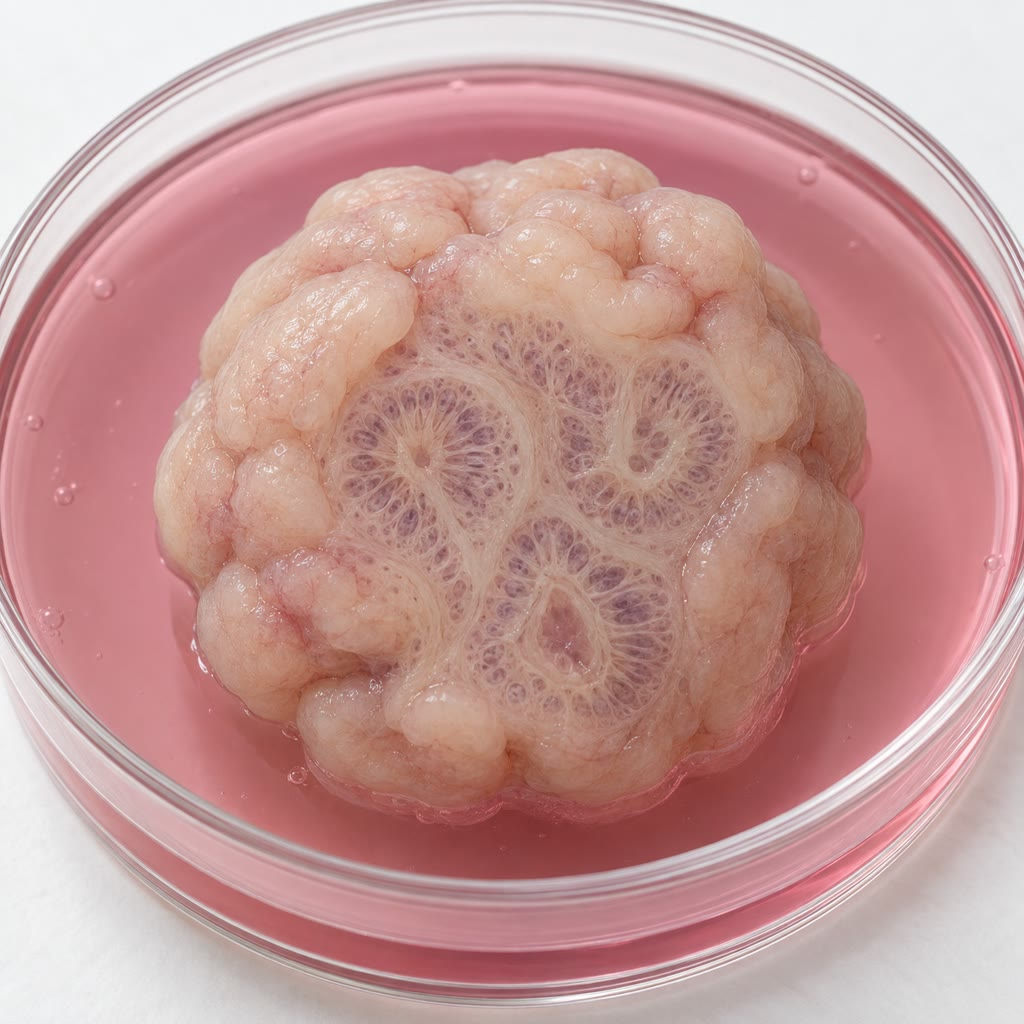
\includegraphics[width=0.4\linewidth]{images/book5/ai/b5-24-brain-organoid.jpg}\hspace{0.04\linewidth}
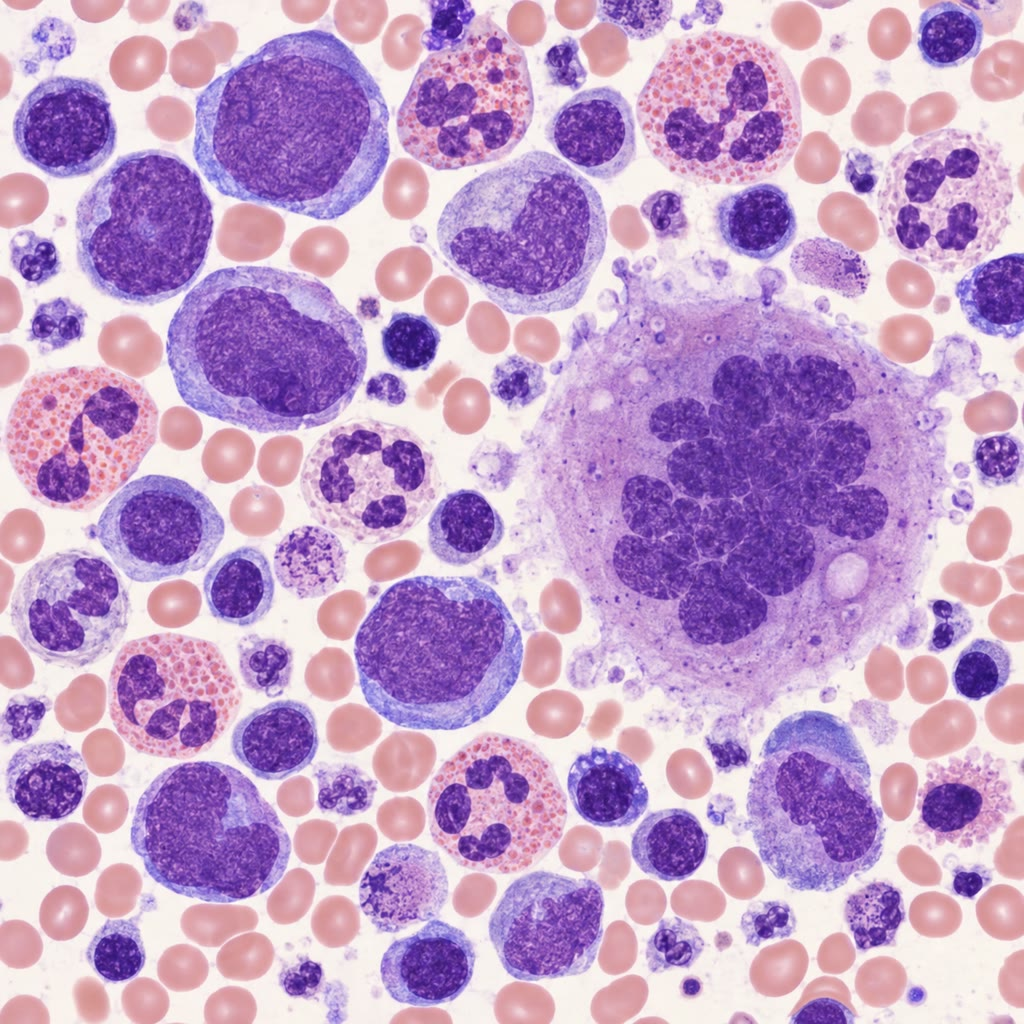
\includegraphics[width=0.4\linewidth]{images/book5/ai/b5-24-bone-marrow-smear.jpg}

{\small 左：由人多能细胞培育的脑\omterm{def:b3:stem-cells:pluripotency}{类器官}
——数毫米大小的自组织类皮层组织，带有
类脑室样腔隙及分层排列的神经元。右：骨髓
涂片，一次展示第一幅图的层级结构：原始细胞、
成熟粒细胞、红细胞前体与巨核细胞。}
\end{omfigure}

\begin{method}[谱系追踪]\label{met:b3:stem-cells:tracing}
\index{谱系追踪}\index{Cre 重组酶}
要确定某组织中哪些细胞是\omterm{def:b3:stem-cells:stem}{干细胞}：（1）选取候选细胞所表达的一个基因，
并将可\omterm{def:b3:developmental-genetics:organiser}{诱导}的重组酶置于其启动子之下
（Cre-ER，仅在给予他莫昔芬时有活性）；
（2）在同一动物中另有一个报告基因，它在
被重组酶切去终止盒后即永久激活——一种
可被所有后代继承的颜色；（3）一次给予
一剂他莫昔芬，在某一时刻标记候选细胞；（4）
定期取组织并对被标记克隆评分：能生长的克隆，
能持续数月且含该组织全部细胞类型者，来自\omterm{def:b3:stem-cells:stem}{干细胞}；
一周内即脱落的克隆，来自
过渡细胞。（5）若用多色报告基因，追踪
克隆之间的竞争。（6）直接检验功能：杀死被标记的细胞，
借助同一启动子驱动表达的毒素受体，观察
该组织是否无法更新。
\end{method}

\section{再生}

\begin{definition}[动物如何再生]\label{def:b3:stem-cells:regeneration}
\index{再生}\index{新生细胞}\index{芽基}\index{去分化}\index{代偿性生长}
再生有三条途径。\emph{Hydra} 与涡虫依靠
成体多能\omterm{def:b3:stem-cells:stem}{干细胞}：涡虫的\emph{新生细胞}，
占其细胞的五分之一，是其唯一的分裂细胞，迁往伤口，
并在位置信号引导下重建任何缺失部分（Wnt
梯度告诉碎片哪一端是尾部；阻断后，尾段
碎片会长出第二个头）。蝾螈借助
\emph{芽基}重建肢体；芽基是残端处分裂细胞形成的帽状结构，主要通过
\emph{去分化}形成：肌纤维碎裂为单核
细胞，软骨与结缔组织细胞回到\omterm{def:b3:stem-cells:stem}{祖细胞}状态，
各自记得其来源组织及在肢体上的位置，
芽基在伤口表皮与神经之下重演胚胎肢体的发育程序，
神经的存在不可或缺（去神经的
残端则无任何生长）。斑马鱼以同样的
方式再生鳍与心脏，心脏中存活的肌细胞分裂，
一个月内替换掉心室的五分之一。哺乳动物很少这样做：肝脏
切除三分之二后仍能恢复其质量，但靠的是原位分裂的剩余细胞
（\emph{代偿性生长}），而不是重建
丢失的肝叶；儿童的指尖可再生；鹿角
每年都从\omterm{def:b3:stem-cells:stem}{干细胞}性骨膜重新生长。为何再生能力不更强，
是一个权衡问题：哺乳动物的创伤反应——迅速凝血，
\omterm{def:b3:innate-immunity:inflammation}{炎症}、成纤维细胞瘢痕——能快速闭合伤口，以防感染
与失血，瘢痕则阻断了芽基；而能
随意去分化并分裂的细胞，可能发展为
\omterm{def:b3:cancer-biology:hallmarks}{癌症}，长寿的温血动物恐难承受这一风险。
\end{definition}

\begin{omfigure}
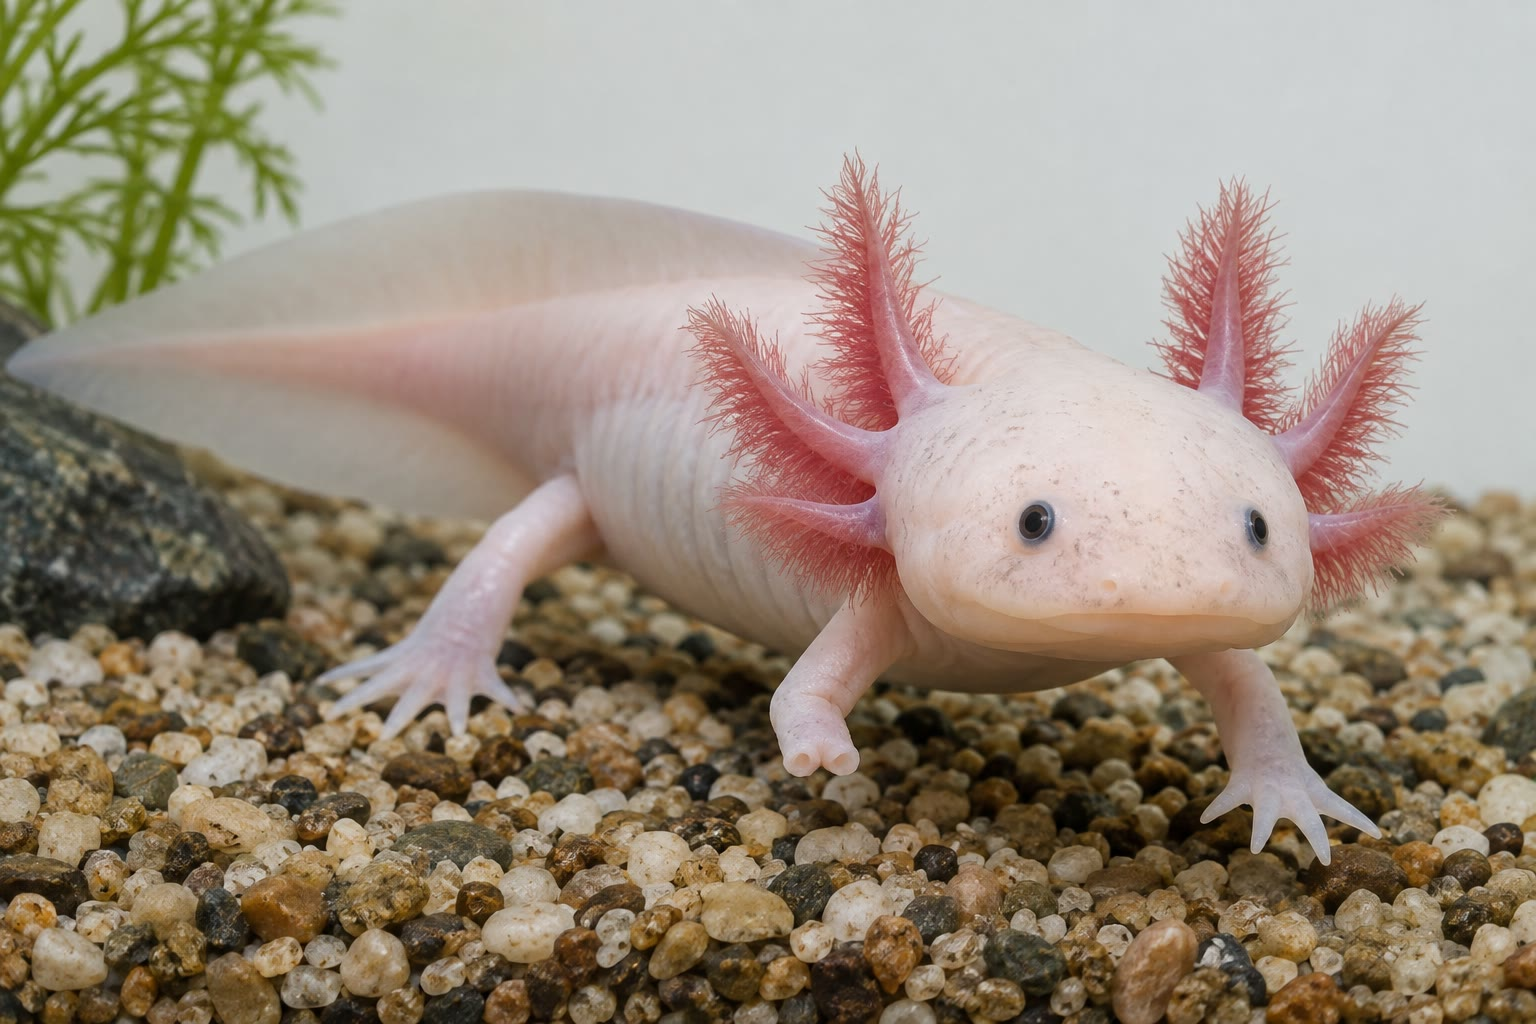
\includegraphics[width=0.46\linewidth]{images/book5/ai/b5-24-axolotl.jpg}\hspace{0.04\linewidth}
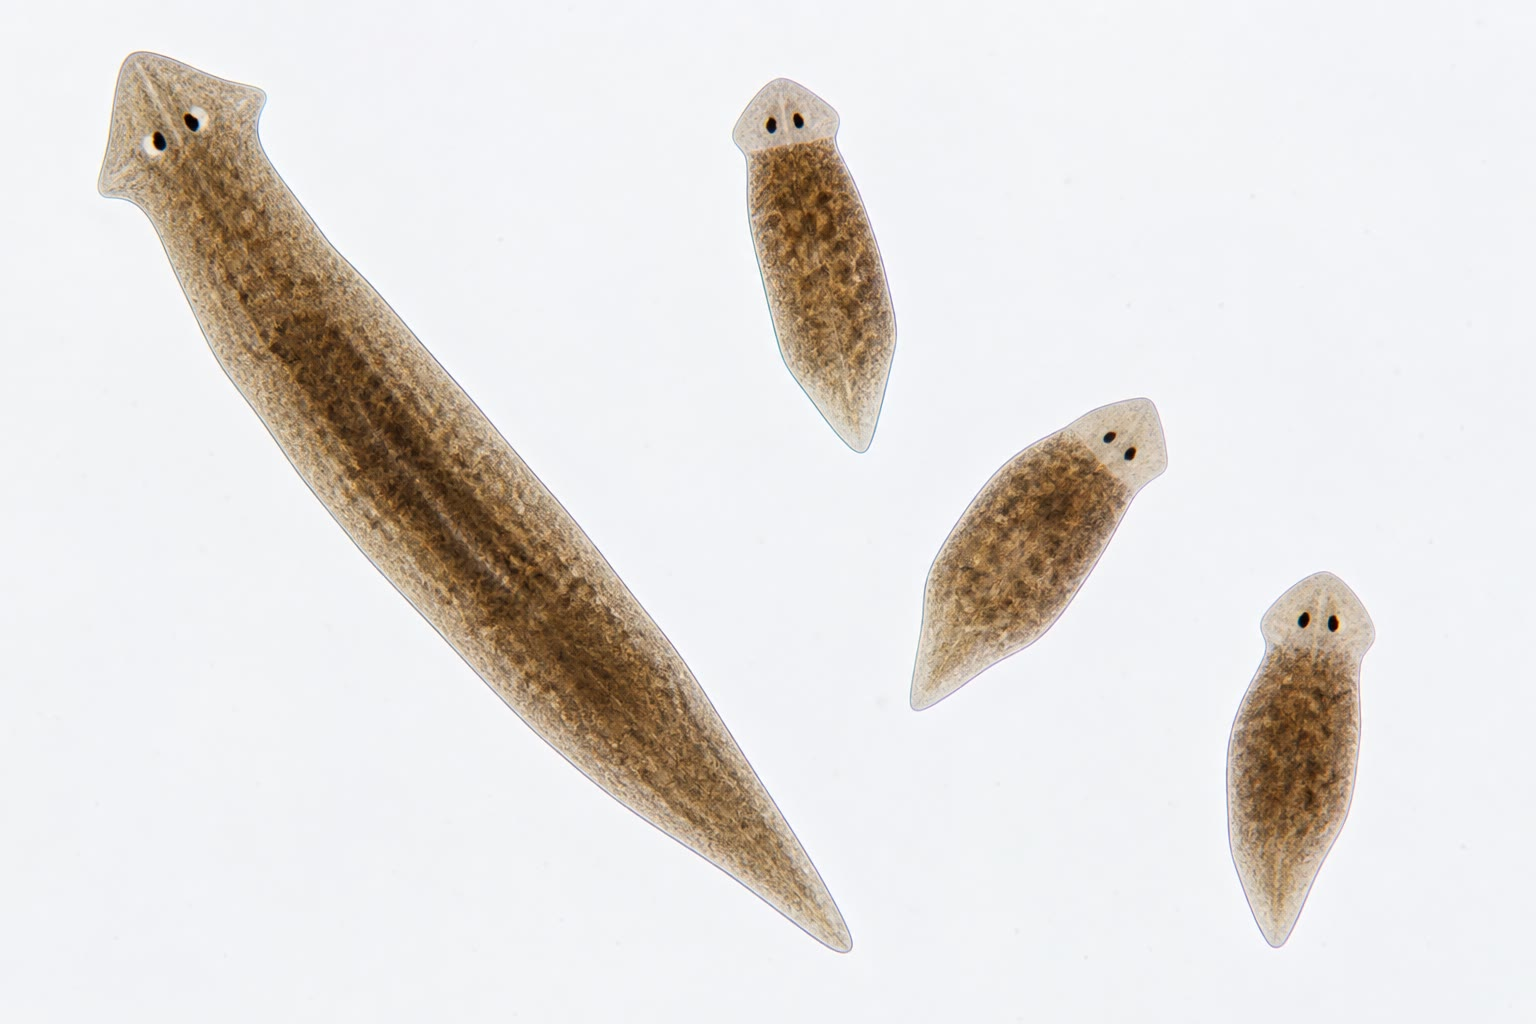
\includegraphics[width=0.46\linewidth]{images/book5/ai/b5-24-planarian-regeneration.jpg}

{\small 左：墨西哥钝口螈，两个月内即可借助\omterm{def:b3:stem-cells:regeneration}{去分化}细胞形成的
\omterm{def:b3:stem-cells:regeneration}{芽基}\omterm{def:b3:stem-cells:regeneration}{再生}出一条肢体，且终生都能如此。右：
被切成若干段的涡虫，每一段均可借助其\omterm{def:b3:stem-cells:regeneration}{新生细胞}
在两周内\omterm{def:b3:stem-cells:regeneration}{再生}出一条完整的虫体。}
\end{omfigure}

\begin{proof}[证据]
摩尔根（1898）将涡虫切成 279 段，发现每一段都能\omterm{def:b3:stem-cells:regeneration}{再生}
出完整的虫体，直至约为身体百分之一大小的极限；雷丁
及其同事（2011）将一个\omterm{def:b3:stem-cells:regeneration}{新生细胞}移植到经致死剂量照射的
虫体中，使其完全恢复——仅一个细胞，便可重建每一种组织。
克拉格尔及其同事（2009）培育出组织逐个被标记为绿色的
墨西哥钝口螈，再将其移植到未标记的宿主体内：截肢之后，绿色
的肌肉只生成肌肉，绿色的软骨只生成软骨——\omterm{def:b3:stem-cells:regeneration}{芽基}
并非多能细胞的池子，而是一群谱系受限的\omterm{def:b3:stem-cells:stem}{祖细胞}的集合，
每一种细胞只\omterm{def:b3:stem-cells:regeneration}{去分化}到其自身组织的\omterm{def:b3:stem-cells:stem}{祖细胞}为止。辛格（1952）
表明，蝾螈的肢体只有在足够数量的神经纤维
抵达断端时才能\omterm{def:b3:stem-cells:regeneration}{再生}；
若将一条神经改道至侧腹的伤口，
那里便会长出一条肢体。
\end{proof}

\section{衰老的算术}

\begin{theorem}[端粒与海弗利克极限]\label{thm:b3:stem-cells:hayflick}
\index{端粒}\index{海弗利克极限}\index{末端复制问题}\index{端粒酶}\index{复制性衰老}
每条染色体都以\emph{\omterm{thm:b3:stem-cells:hayflick}{端粒}}结尾，\omterm{thm:b3:stem-cells:hayflick}{端粒}由数千个碱基对的
TTAGGG 重复序列组成。由于 DNA 聚合酶无法完成后随链的
最后一段（即\emph{末端复制问题}），每次分裂都使
每个\omterm{thm:b3:stem-cells:hayflick}{端粒}缩短 $\Delta \approx$ \qtyrange{50}{100}{bp}。
设 $L_{0} \approx \qty{10}{kb}$，并触发
\emph{\omterm{thm:b3:stem-cells:hayflick}{复制性衰老}}——一种永久性的、由 \omterm{def:b3:cancer-biology:genes}{p53} 强制施行的停滞——
当最短\omterm{thm:b3:stem-cells:hayflick}{端粒}达到 $L_{\mathrm{crit}} \approx \qty{4}{kb}$ 时，
一个细胞谱系至多可分裂
\[
n_{\max} = \frac{L_{0} - L_{\mathrm{crit}}}{\Delta} \approx \frac{6000}{50\text{--}100} \approx 60\text{--}120
\]
次：这便是\emph{\omterm{thm:b3:stem-cells:hayflick}{海弗利克极限}}，即人类成纤维细胞在培养中
停止之前所能完成的五十余次群体倍增。
\emph{\omterm{def:b3:cancer-biology:telomerase}{端粒酶}}是一种以 RNA 为模板的逆转录酶，
使\omterm{thm:b3:stem-cells:hayflick}{端粒}末端重新延长；它在种系细胞、\omterm{def:b3:stem-cells:pluripotency}{胚胎干细胞}以及许多
成体\omterm{def:b3:stem-cells:stem}{干细胞}中活跃，也存在于 \qty{90}{\%} 的\omterm{def:b3:cancer-biology:hallmarks}{癌症}中，
这些癌细胞正是通过重新开启\omterm{def:b3:cancer-biology:telomerase}{端粒酶}而摆脱了这一极限。若一个\omterm{def:b3:stem-cells:stem}{干细胞}
每年分裂 $d$ 次，且\omterm{def:b3:cancer-biology:telomerase}{端粒酶}补偿了损失的比例 $f$，则
其分裂次数为 $n_{\max} = (L_{0} - L_{\mathrm{crit}})/[(1 - f)\Delta]$，
寿命为 $n_{\max}/d$ 年：取 $f = 0.7$、$\Delta
= 60$、$d = 1$，造血\omterm{def:b3:stem-cells:stem}{干细胞}可存活约 330 年——
但其\omterm{def:b3:stem-cells:stem}{祖细胞}在\omterm{def:b3:cancer-biology:telomerase}{端粒酶}关闭的情况下，至一个红细胞仅有二十次分裂，
每经过一个谱系阶段便耗去其储备的五分之一，这正是老年人的血细胞
\omterm{thm:b3:stem-cells:hayflick}{端粒}比年轻人短的原因；
每年约短 \qty{30}{bp}。
\end{theorem}
\begin{proof}
每次分裂的损失是固定长度，因此\omterm{thm:b3:stem-cells:hayflick}{端粒}长度随分裂次数
线性下降，即 $L_{n} = L_{0} - n\Delta$，并
达到 $L_{\mathrm{crit}}$，对应 $n = (L_{0} - L_{\mathrm{crit}})/\Delta$；若
存在部分补偿，则每次分裂的净损失为 $(1 - f)\Delta$。
海弗利克与穆尔黑德（1961）表明，正常人类成纤维细胞在
约五十次倍增后停止，无论培养条件如何；
在二十次倍增后冷冻并复苏的细胞，只能再完成
剩余的三十次——它们计数的是分裂次数而非时间——而且
来自老年供体的细胞，其极限更低。哈利、富特彻与格雷德
（1990）测量了\omterm{thm:b3:stem-cells:hayflick}{端粒}随培养中倍增次数以及供体年龄而缩短的情况；
博德纳及其同事（1998）将\omterm{def:b3:cancer-biology:telomerase}{端粒酶}导入正常细胞，
这些细胞便可无限地越过极限继续分裂，且并未成为癌细胞，
由此确立了\omterm{thm:b3:stem-cells:hayflick}{端粒}作为分裂计时钟的地位。
\end{proof}

\begin{omfigure}
\begin{tikzpicture}
\begin{axis}[
  width=0.62\linewidth, height=5.4cm,
  axis x line=bottom, axis y line=left,
  xmin=0, xmax=120, ymin=0, ymax=11,
  xlabel={群体倍增次数}, ylabel={端粒长度（kb）},
  xlabel style={font=\small, at={(axis description cs:0.5,-0.12)}, anchor=north}, ylabel style={font=\small},
  tick label style={font=\small}, xtick={0,30,60,90,120}, ytick={4,7,10},
  clip=false,
]
\addplot[very thick, omDef, domain=0:60, samples=2] {10-0.1*x};
\addplot[very thick, omThm, domain=0:120, samples=2] {10-0.05*x};
\addplot[very thick, omMeth!70!black, domain=0:120, samples=2] {10-0.015*x};
\draw[dashed, gray] (axis cs:0,4) -- (axis cs:120,4); \node[font=\scriptsize, gray, anchor=north west] at (axis cs:2,3.9) {$L_{\mathrm{crit}} = \qty{4}{kb}$ 处衰老};
\node[font=\scriptsize, omDef, anchor=south west] at (axis cs:63,4.3) {$\Delta = \qty{100}{bp}$：60 次倍增};
\node[font=\scriptsize, omThm, anchor=west] at (axis cs:70,8.0) {$\Delta = \qty{50}{bp}$：120 次};
\node[font=\scriptsize, omMeth!70!black, anchor=south west, align=left] at (axis cs:78,9.3) {端粒酶补偿 \\\qty{70}{\%}：400 次};
\fill[omDef] (axis cs:60,4) circle (2pt); \fill[omThm] (axis cs:120,4) circle (2pt);
\end{axis}
\end{tikzpicture}

{\small \omterm{thm:b3:stem-cells:hayflick}{端粒}作为分裂计数器。每次分裂的损失量固定，图像呈一条直线；
与临界长度相交之处，即该谱系停止分裂的位置。
\omterm{def:b3:cancer-biology:telomerase}{端粒酶}使斜率变缓；完全激活时则消除这一极限——
见于种系细胞与癌细胞中。}
\end{omfigure}

\begin{proposition}[冈珀茨定律]\label{prop:b3:stem-cells:gompertz}
\index{冈珀茨定律}\index{死亡率}\index{衰老特征}\index{衰老细胞}
三十岁以上，人类的\omterm{prop:b3:stem-cells:gompertz}{死亡率} $\mu(t)$——即下一年内死亡的概率——
每八年翻一番：$\mu(t) =
\mu_{0}\,\mathrm{e}^{\gamma(t - t_{0})}$，其中 $\gamma = \ln 2/8 \approx
\qty{0.087}{yr^{-1}}$（冈珀茨，1825）。于是存活到年龄 $t$ 的概率为
\[
S(t) = \exp\!\Bigl[-\frac{\mu_{0}}{\gamma}\bigl(\mathrm{e}^{\gamma(t - t_{0})} - 1\bigr)\Bigr],
\]
曲线在数十年间近乎平坦，随后急剧下降，其中位
寿命为 $t_{1/2} = t_{0} + \gamma^{-1}\ln(1 + \gamma\ln 2/\mu_{0})$：
若三十岁时 $\mu_{0} = 10^{-3}$（每年），则约为 $30 + 47 = 77$ 岁。
同一定律在常数不同的情况下，也适用于小鼠（倍增时间
三个月）、狗、果蝇和线虫：\omterm{def:b3:cell-cycle-apoptosis:other}{衰老}即脆弱性的指数上升，
而非一只会停摆的时钟。指数背后的生物学机制
是一组相互作用的\emph{\omterm{prop:b3:stem-cells:gompertz}{衰老特征}}：DNA \omterm{def:b3:dna-repair:lesions}{损伤}的累积与
表观遗传漂移、\omterm{thm:b3:stem-cells:hayflick}{端粒}损耗、蛋白质稳态丧失、
线粒体功能衰退、\omterm{def:b3:stem-cells:stem}{干细胞}库耗竭，以及
\emph{\omterm{prop:b3:stem-cells:gompertz}{衰老细胞}}的积累，这些细胞不再分裂，却会分泌
\omterm{def:b3:innate-immunity:inflammation}{炎症}信号，以及慢性\omterm{def:b3:innate-immunity:inflammation}{炎症}；在小鼠中，清除
\omterm{prop:b3:stem-cells:gompertz}{衰老细胞}或限制热量摄入可延长寿命，在线虫中，
\omterm{def:b3:endocrinology:glucose}{胰岛素}样通路中的单个突变可使寿命翻倍。人类的指数能否降低，
而非常数 $\mu_{0}$，
医学已在一个世纪内将其降低了十倍，这仍是一个悬而未决的问题。
\end{proposition}
\begin{proof}
若 $\mu$ 为风险率，则 $\mathrm{d}S/\mathrm{d}t = -\mu(t)S$，于是 $\ln S =
-\int_{t_{0}}^{t}\mu = -(\mu_{0}/\gamma)(\mathrm{e}^{\gamma(t-t_{0})} -
1)$。令 $S = 1/2$，得 $\mathrm{e}^{\gamma(t-t_{0})} = 1 + \gamma\ln 2/
\mu_{0}$，由此得中位寿命；取 $\gamma = 0.087$ 与 $\mu_{0} =
10^{-3}$，$\ln(1 + 60) = 4.1$，$t - t_{0} = 47$。经验定律是
冈珀茨对英文生命表的拟合；它能描述如此多的
物种共有相同形式、常数因物种而异，这一点在本阶段不加证明地承认，
仅作为一个世纪人口统计学研究的总结。
\end{proof}

\begin{omfigure}
\begin{tikzpicture}
\begin{semilogyaxis}[
  width=0.5\linewidth, height=5.2cm,
  axis x line=bottom, axis y line=left,
  xmin=20, xmax=100, ymin=0.0003, ymax=1,
  xlabel={年龄（年）}, ylabel={每年死亡率},
  xlabel style={font=\small, at={(axis description cs:0.5,-0.12)}, anchor=north}, ylabel style={font=\small},
  tick label style={font=\small}, xtick={30,50,70,90}, ytick={0.001,0.01,0.1,1}, yticklabels={0.001,0.01,0.1,1},
  clip=false,
]
\addplot[very thick, omDef, domain=30:100, samples=2] {0.001*exp(0.0866*(x-30))};
\node[font=\scriptsize, omDef, anchor=north west, align=left] at (axis cs:32,0.3) {$\mu = \mu_{0}\,\mathrm{e}^{\gamma(t-30)}$\\每 8 年翻一番};
\end{semilogyaxis}
\begin{axis}[
  at={(0.55\linewidth,0)}, anchor=south west,
  width=0.43\linewidth, height=5.2cm,
  axis x line=bottom, axis y line=left,
  xmin=20, xmax=110, ymin=0, ymax=1.05,
  xlabel={年龄（年）}, ylabel={存活比例},
  xlabel style={font=\small, at={(axis description cs:0.5,-0.12)}, anchor=north}, ylabel style={font=\small},
  tick label style={font=\small}, xtick={30,50,77,100}, ytick={0.5,1},
  clip=false,
]
\addplot[very thick, omThm, domain=30:110, samples=80] {exp(-(0.001/0.0866)*(exp(0.0866*(x-30))-1))};
\draw[dashed, gray] (axis cs:77,0) -- (axis cs:77,0.5) -- (axis cs:20,0.5);
\node[font=\scriptsize, omThm, anchor=north east, align=right] at (axis cs:75,0.45) {中位寿命 \\77 年};
\end{axis}
\end{tikzpicture}

{\small 冈珀茨定律。左图：以对数坐标作纵轴时，\omterm{prop:b3:stem-cells:gompertz}{死亡率}
自三十岁起便是一条直线。右图：随之而来的生存曲线，
先为平台，随后陡降，中位寿命位于风险率的
积分达到 $\ln 2$ 之处。}
\end{omfigure}

\begin{remark}[更新及其代价]\label{rem:b3:stem-cells:remark}
能够\omterm{def:b3:stem-cells:stem}{自我更新}的机体，必须保有能无限分裂的细胞，
而能无限分裂的细胞恰恰是\omterm{def:b3:cancer-biology:hallmarks}{癌症}的原料；
机体若靠计算分裂次数并强制\omterm{def:b3:cell-cycle-apoptosis:other}{衰老}来防癌，
久而久之必将耗尽可分裂的细胞。
\omterm{def:b3:stem-cells:stem}{干细胞}层级是一种解决办法——少数缓慢分裂的细胞受
\omterm{def:b3:stem-cells:stem}{生态位}保护，大量快速细胞很快死去；\omterm{thm:b3:stem-cells:hayflick}{海弗利克极限}则是另一种办法，
而冈珀茨的指数项正是它们代价的总和。
蝾螈则另有代价：它容忍细胞\omterm{def:b3:stem-cells:regeneration}{去分化}，
并能\omterm{def:b3:stem-cells:regeneration}{再生}肢体；它是变温动物，生长缓慢，很少活得足够久，
以至于承担不起\omterm{def:b3:cancer-biology:hallmarks}{癌症}的代价。你出生时具有的细胞，
大部分已不再是你现在的细胞；而那些制造出替代细胞的，
才是你必须保留的细胞。
\end{remark}

\section{练习}

\begin{exercise}[$\star$]\label{exo:b3:stem-cells:1}
给出\omterm{def:b3:stem-cells:stem}{自我更新}、潜能、\omterm{def:b3:stem-cells:stem}{生态位}与\omterm{def:b3:stem-cells:stem}{过渡放大细胞}的定义，
并各举一个肠道中的例子。
\end{exercise}

\begin{exercise}[$\star$]\label{exo:b3:stem-cells:2}
脾集落实验说明了什么？\omterm{def:b3:stem-cells:stem}{干细胞}的哪一种性质
需要第二只小鼠才能证明？
\end{exercise}

\begin{exercise}[$\star$]\label{exo:b3:stem-cells:3}
写出四种山中因子，并解释\omterm{def:b3:stem-cells:pluripotency}{重编程}为何需要数周，
且仅能在千分之一的细胞中成功。
\end{exercise}

\begin{exercise}[$\star$]\label{exo:b3:stem-cells:4}
比较涡虫与蝾螈的\omterm{def:b3:stem-cells:regeneration}{再生}途径，
并说明克拉格尔的移植实验关于\omterm{def:b3:stem-cells:regeneration}{芽基}揭示了什么。
\end{exercise}

\begin{exercise}[$\star\star$]\label{exo:b3:stem-cells:5}
\omterm{thm:b3:stem-cells:hayflick}{端粒}起始长度为 \qty{11}{kb}，\omterm{def:b3:cell-cycle-apoptosis:other}{衰老}界限为 \qty{5}{kb}，
每次分裂损失 \qty{75}{bp}。\omterm{thm:b3:stem-cells:hayflick}{海弗利克极限}为多少？
来自 70 岁供体的细胞\omterm{thm:b3:stem-cells:hayflick}{端粒}为 \qty{8}{kb}：尚余多少次倍增？若\omterm{def:b3:cancer-biology:telomerase}{端粒酶}
可补偿损失的 \qty{60}{\%}，则极限为多少？
\end{exercise}

\begin{exercise}[$\star\star$]\label{exo:b3:stem-cells:6}
一个\omterm{prop:b3:stem-cells:crypt}{隐窝}中有 14 个\omterm{def:b3:stem-cells:stem}{干细胞}，每天分裂一次，并为过渡细胞提供来源，
这些过渡细胞再分裂 4 次，\omterm{prop:b3:stem-cells:crypt}{隐窝}每天
向其绒毛供应 \num{300} 个细胞。请核算：每天有多少次\omterm{def:b3:stem-cells:stem}{干细胞}分裂
会产生分化的子细胞，并且这相当于多少个\omterm{def:b3:stem-cells:stem}{干细胞}的
分裂量？
\end{exercise}

\begin{exercise}[$\star\star$]\label{exo:b3:stem-cells:7}
人体每天生成 $2\times 10^{11}$ 个红细胞，每个都是
由一个\omterm{def:b3:stem-cells:stem}{干细胞}经约 20 次分裂产生。每天需要多少次\omterm{def:b3:stem-cells:stem}{干细胞}分裂，
若有 \num{10000} 个\omterm{def:b3:stem-cells:stem}{干细胞}，每个\omterm{def:b3:stem-cells:stem}{干细胞}平均多久分裂一次？
与观察到的“约每年一次”相比较，并解释
其中的差异。
\end{exercise}

\begin{exercise}[$\star\star$]\label{exo:b3:stem-cells:8}
取 $\gamma = \qty{0.087}{yr^{-1}}$，$\mu_{0} = 10^{-3}$（三十岁时），
计算 50、70 和 90 岁时的\omterm{prop:b3:stem-cells:gompertz}{死亡率}，70 岁和 90 岁时的存活率，以及
中位寿命。将 $\mu_{0}$ 减半会对中位寿命产生什么影响？
将 $\gamma$ 减半又有什么影响？
\end{exercise}

\begin{exercise}[$\star\star$]\label{exo:b3:stem-cells:9}
切除大鼠肝脏的三分之二。余下的肝细胞全部都能分裂，
它们可在十天内恢复肝脏的质量。每个肝细胞需要分裂多少次？
为何称之为\omterm{def:b3:stem-cells:regeneration}{代偿性生长}而非\omterm{def:b3:stem-cells:regeneration}{再生}？
并说明肝脏\emph{不}重建什么？
\end{exercise}

\begin{exercise}[$\star\star\star$]\label{exo:b3:stem-cells:10}
\omterm{prop:b3:stem-cells:crypt}{中性漂变}：\omterm{def:b3:stem-cells:stem}{生态位}中的 $N$ 个\omterm{def:b3:stem-cells:stem}{干细胞}进行对称分裂；每次
事件中，一个细胞分裂，另一个随机丢失，因此某一克隆的细胞数在
$0$ 与 $N$ 之间作随机游走。论证：由
$k$ 个细胞组成的克隆最终占据\omterm{def:b3:stem-cells:stem}{生态位}的概率为
$k/N$，并说明当 $N = 14$ 时，单细胞克隆的概率为 $1/14$。
这对携带新
中性突变的\omterm{def:b3:stem-cells:stem}{干细胞}的命运有何预测？
\end{exercise}

\begin{exercise}[$\star\star\star$]\label{exo:b3:stem-cells:11}
某突变使\omterm{def:b3:stem-cells:stem}{干细胞}克隆在
\cref{exo:b3:stem-cells:10}的竞争中获得 \qty{10}{\%} 的优势。定性解释其占据
概率为何远高于 $k/N$，为何老年人的\omterm{prop:b3:stem-cells:crypt}{隐窝}与骨髓日益
被少数克隆占据（克隆性造血），
以及这为何是迈向\omterm{def:b3:cancer-biology:hallmarks}{癌症}的第一步，
但本身并非\omterm{def:b3:cancer-biology:hallmarks}{癌症}。
\end{exercise}

\begin{exercise}[$\star\star\star$]\label{exo:b3:stem-cells:12}
假设 Gompertz 指数 $\gamma$ 反映\omterm{def:b3:dna-repair:lesions}{损伤}累积的速率，常数 $\mu_{0}$ 反映环境。
自 1900 年以来，医学使 $\mu_{0}$ 降低了十倍，而 $\gamma$ 未变。
计算这一十倍降低带来的中位寿命增益，
以及再降低十倍的进一步增益；
解释收益为何递减，以及
$\gamma$ 降低 \qty{20}{\%} 会带来何种不同的影响。
\end{exercise}

\section{问题：你出生时拥有的细胞}

\begin{problem}[{周末问题——数字中的身体更新：血液的层级
及其对干细胞的要求，隐窝的漂变，
端粒时钟，以及端粒酶与祖细胞如何消耗它，
种群的 Gompertz 曲线，以及再生动物所接受的权衡，
最终归结为 Hayflick 次数、干细胞的终身
储备与中位寿命}]
\label{pb:b3:stem-cells:1}
数据：红细胞每天 $2.5\times 10^{11}$ 个，粒细胞每天 $10^{11}$ 个；
从\omterm{def:b3:stem-cells:stem}{干细胞}到成熟细胞需 $20$ 次分裂；造血\omterm{def:b3:stem-cells:stem}{干细胞}
数为 \num{10000} 个。\omterm{thm:b3:stem-cells:hayflick}{端粒}：$L_{0} = \qty{10}{kb}$，
$L_{\mathrm{crit}} = \qty{4}{kb}$，$\Delta = \qty{60}{bp}$ 每次分裂；
\omterm{def:b3:stem-cells:stem}{干细胞}中的\omterm{def:b3:cancer-biology:telomerase}{端粒酶}补偿 $f = 0.7$；\omterm{def:b3:stem-cells:stem}{祖细胞}中无\omterm{def:b3:cancer-biology:telomerase}{端粒酶}。
\omterm{prop:b3:stem-cells:crypt}{隐窝}：$N = 14$ 个\omterm{def:b3:stem-cells:stem}{干细胞}，每天分裂一次。Gompertz：$\mu_{0} =
10^{-3}$ 每年，在 30 岁时；$\gamma = \qty{0.087}{yr^{-1}}$。蝾螈
肢体：\qty{40}{mm} 在 \qty{60}{d} 内\omterm{def:b3:stem-cells:regeneration}{再生}；\omterm{def:b3:stem-cells:regeneration}{芽基}由 $10^{5}$ 个细胞
增长至 $10^{8}$ 个。

\medskip
\noindent\textbf{第一部分——血液。}
\begin{enumerate}
  \item 每天产生的细胞总数，以及每秒产生的细胞数。
  \item 每个成熟细胞是 $20$ 次分裂的终点：由一个\omterm{def:b3:stem-cells:stem}{干细胞}的定向子细胞
        可产生多少个细胞？每天需要多少
        个定向子细胞？
  \item 若有 \num{10000} 个\omterm{def:b3:stem-cells:stem}{干细胞}，则每个\omterm{def:b3:stem-cells:stem}{干细胞}每天意味着
        多少次分化分裂？每年又是多少？
  \item 实测\omterm{def:b3:stem-cells:stem}{干细胞}约每年分裂一次。请调和二者：\omterm{def:b3:stem-cells:stem}{祖细胞}必须做什么，
        才能使第~3 题计算中假设由\omterm{def:b3:stem-cells:stem}{干细胞}完成的工作
        得以实现？
  \item \omterm{def:b3:stem-cells:stem}{祖细胞}没有\omterm{def:b3:cancer-biology:telomerase}{端粒酶}。从 \qty{10}{kb} 出发，红细胞前体经过
        $20$ 次分裂后\omterm{thm:b3:stem-cells:hayflick}{端粒}长度达到多少？
        它高于 $L_{\mathrm{crit}}$，这有关系吗？
  \item 一个\omterm{def:b3:stem-cells:stem}{干细胞}每年分裂一次，$f = 0.7$：每次分裂的净损失，
        直至\omterm{def:b3:cell-cycle-apoptosis:other}{衰老}的分裂次数及年数。请评论。
\end{enumerate}

\medskip
\noindent\textbf{第二部分——\omterm{prop:b3:stem-cells:crypt}{隐窝}。}
\begin{enumerate}[resume]
  \item \omterm{def:b3:stem-cells:stem}{干细胞}层每个\omterm{prop:b3:stem-cells:crypt}{隐窝}每天的分裂次数；若一半事件补充丢失的\omterm{def:b3:stem-cells:stem}{干细胞}，
        另一半补充过渡区，则每天产生多少个定向细胞，
        以及经过 $4$ 次过渡分裂后产生多少个
        绒\omterm{def:b3:sensory-systems:cochlea}{毛细胞}？
  \item 单细胞克隆的占据概率为 $1/N$。达到单克隆化的期望时间
        约为每个细胞 $N^{2}$ 次分裂事件的量级；请以天估算，
        并与“彩纸屑”标记的观察结果比较，
        后者以月计。
  \item 一个\omterm{def:b3:stem-cells:stem}{干细胞}获得突变。其最终在\omterm{prop:b3:stem-cells:crypt}{隐窝}中固定的概率为多少？
        若每个\omterm{prop:b3:stem-cells:crypt}{隐窝}产生一次突变，则结肠的 $10^{7}$ 个\omterm{prop:b3:stem-cells:crypt}{隐窝}中
        有多少个会使突变固定？
  \item 为何\omterm{prop:b3:stem-cells:crypt}{隐窝}的漂变比每个\omterm{def:b3:stem-cells:stem}{干细胞}终身\omterm{def:b3:stem-cells:stem}{不对称分裂}的组织
        更能防癌？
  \item 照射杀死\omterm{def:b3:stem-cells:stem}{干细胞}后，过渡细胞发生逆转，
        重新填充\omterm{def:b3:stem-cells:stem}{生态位}。这说明
        干性存在于何处？
  \item 勾勒区分对称漂变与\omterm{def:b3:stem-cells:stem}{不对称分裂}的\omterm{met:b3:stem-cells:tracing}{谱系追踪}实验，
        并给出两种结果。
\end{enumerate}

\medskip
\noindent\textbf{第三部分——时钟。}
\begin{enumerate}[resume]
  \item 无\omterm{def:b3:cancer-biology:telomerase}{端粒酶}的体细胞谱系的 Hayflick 极限。
  \item 成纤维细胞培养物在 $25$ 次倍增后冷冻，
        十年后解冻：还剩多少次倍增？这说明
        细胞计数的是什么？
  \item 成人白细胞\omterm{thm:b3:stem-cells:hayflick}{端粒}每年缩短 \qty{30}{bp}。从二十岁时的 \qty{8}{kb} 起算，
        何时达到 $L_{\mathrm{crit}}$？
        与寿命比较并评论。
  \item 将\omterm{def:b3:cancer-biology:telomerase}{端粒酶}导入正常成纤维细胞，使其越过极限
        而不致癌。\omterm{def:b3:cancer-biology:telomerase}{端粒酶}在 \qty{90}{\%} 的
        \omterm{def:b3:cancer-biology:hallmarks}{癌症}中活跃。请调和这两种说法。
  \item 计算 40、60、80 和 100 岁时的 Gompertz \omterm{prop:b3:stem-cells:gompertz}{死亡率}，以及
        存活到各年龄的比例。
  \item 中位寿命；以及 \qty{10}{\%} 个体存活的年龄。
\end{enumerate}

\medskip
\noindent\textbf{第四部分——\omterm{def:b3:stem-cells:regeneration}{再生}。}
\begin{enumerate}[resume]
  \item 蝾螈：以 mm/天计的平均\omterm{def:b3:stem-cells:regeneration}{再生}速率；
        \omterm{def:b3:stem-cells:regeneration}{芽基}由 $10^{5}$ 增长至 $10^{8}$ 个细胞所需的倍增次数，
        以及 60 天内的平均倍增时间。
  \item 若\omterm{def:b3:stem-cells:regeneration}{去分化}细胞终生像\omterm{def:b3:stem-cells:regeneration}{芽基}细胞那样分裂，
        且每次分裂中每个细胞产生致癌突变的概率为 $10^{-9}$，
        则一次\omterm{def:b3:stem-cells:regeneration}{再生}中会产生多少个此类突变？
        为何蝾螈几乎从不致癌，
        而哺乳动物却可能无法侥幸逃脱？
  \item 去神经支配使断端的\omterm{def:b3:stem-cells:regeneration}{再生}停止。请设计一个实验，
        证明神经提供一种可扩散的因子，
        并给出该因子的一种可能身份。
  \item 涡虫的尾段长出的是第二条尾巴而非头部，
        这发生于 Wnt 抑制剂被\omterm{met:b3:rna-regulation:knockdown}{敲低}时。请结合梯度
        与该尾段的位置记忆加以解释。
  \item 人肝经三分之二切除后：需有多少比例的肝细胞分裂一次，
        或分裂两次，方能恢复肝脏质量？
        为何结果是一个有功能但形状错误的肝脏？
  \item 若身体像蝾螈那样\omterm{def:b3:stem-cells:regeneration}{再生}，为何其 Gompertz 曲线会不同？
        朝哪个方向变化？
  \item 总结：Hayflick 次数（问题~13）、\omterm{def:b3:cancer-biology:telomerase}{端粒酶}辅助的\omterm{def:b3:stem-cells:stem}{干细胞}
        分裂次数及年数（问题~6），以及
        中位寿命（问题~18）。
\end{enumerate}
\end{problem}
